\documentclass[12pt,a4paper,ngerman]{scrartcl}

\usepackage[ngerman]{babel}
\usepackage[utf8]{inputenc}
\usepackage[T1]{fontenc}
\usepackage{csquotes}
\usepackage{graphicx}


\author{Thomas Hilarius Meyer\\ \textsf{thomas.hilarius.meyer@gmail.com}}
\title{Die Gersheimer Schulimkerei-Beute (GSIB)}
\subtitle{Überlegungen zu Konzeption, Bau und Betriebsweise}


\begin{document}
	\maketitle

        
\begin{abstract}
	Die Gersheimer Schulimkerei-Beute (GSIB) ist eine Trogbeute für 24 Zander-Rähmchen.
	Sie eignet sich besonders für den pädagogischen Umgang mit Bienen, da alle Waben in einer
	Ebene liegen und somit direkt einsehbar und zugänglich sind; im Umgang mit ihr sind
	keine schweren Gewichte zu heben und die Arbeitshöhe bleibt konstant.
	Alle Verfahren der modernen Magazin-Imkerei lassen sich mit der GSIB durchführen und
	ein späterer Wechsel der Jungimker etwa zur Liebigbeute ist problemlos möglich.
\end{abstract}


\section{Gestaltungsprinzipien}

Die Zeit ist reif für einen neuen Bienenkasten, der speziell auf die Bedürfnisse einer Schulimkerei und ihrer Mitglieder --
besonders in den ersten 1--2 Jahren des Imkern-Lernens -- ausgelegt ist!

Die Mitglieder der Schulimkerei Gersheim haben eine Bienenbeute entwickelt, die sich ausschließlich diesem Ziel widmet:
die Gersheimer Schulimkerei-Beute (GSIB).

Nach einem angemessenen Erprobungsbetrieb könnte die Herstellung der GSIB die Angebotspalette unserer Schüllerfirma
entscheidend erweitern.


\subsection{Vorüberlegungen / Anforderungen}

Was müsste ein Schulbienenkasten besser können als die Liebig-Beute?

\begin{enumerate}
\item Die Imkerneulinge sollen keine Zargen abheben müssen, denn dies bedeutet...
  \begin{itemize}
  \item eine Frage der Kraft,
  \item ist eine psychologische Hemmschwelle
  \item  und eine Störung der Bienen.
  \end{itemize}
\item Alle Teile des Bienenstocks sollen gleichzeitig sichtbar sein (von oben, auf einen Blick),
\item das Wabenmaß soll das weit verbreitete Zandermaß sein,
  um später leichter auf Magazinbeuten umsteigen zu können (eine Beute, aus der man \enquote{herauswächst}...),
\item die Betriebsweise soll sehr nahe an der Magazinimkerei liegen (imkern lernen) und
\item der Bau soll zu einem geringen Preis und
\item mit wenig Aufwand möglich sein.
\end{enumerate}

In Kauf genommene Nachteile sind weitgehend irrelevant für den speziellen Zweck der \enquote{pädagogischen} Bienenbeute:

\begin{itemize}
\item \enquote{Unwirtschaftliches} Arbeiten (\enquote{wabenweise} statt \enquote{zargenweise}) -- es geht nicht um Erwerbsbienenhaltung,
  sondern um pädagogisch orientiertes Imkern.
\item Schwieriges Wandern wegen des hohen Beuten-Gewichts -- eine Schulimkerei ist erfahrungsgemäß immer eine Standimkerei.
\end{itemize}


\subsection{Konkrete Designentscheidungen}

Folgende Konstruktionsentscheidungen sind für den Entwurf maßgeblich:

\begin{itemize}
\item Zander-Rähmchen als verbreitetstes Rähmchenmaß,
\item gleiches Maß im Brut- und Honigraum,
\item vertikales Königinnenabsperrgitter möglich,
\item Möglichkeit einer vertikalen Bienenflucht,
\item extrem leichter Zusammenbau aus wenigen, einfachen Teilen.
\end{itemize}


\section{Bisherige Ansätze}

Welche Bienenkästen mit grundsätzlich ähnlicher Konstruktion (Waben auf einer Ebene) gibt es schon und warum sind diese
für die speziellen Zwecke einer Schulimkerei nicht oder nicht optimal geeignet?

\begin{description}
\item[Hohenheimer Einfachbeute] ideales System für \enquote{erwachsene} Imker; doch Nachteil: schweres Heben, Scheu des Zargen-Abhebens...
\item[Golzbeute] komplizierter Aufbau, teuer, spezielles Wabenmaß (Kuntzsch hoch), keine Bienenflucht.
\item[Mellifera Einraumbeute] spezielles Wabenmaß, kein Abspergitter und keine Bienenflucht möglich.
\item[Top-Bar-Hive] Umstieg auf Magazin-Imkerei sehr kompliziert.
\item[Bienenkiste] extrem unergonomisch; Stabilbau verhindert Wabenkontrolle.
\item[Kunesa-Beute]
\item[BienenBox] Format Kuntzsch (hoch)  (www.bienenbox.de)
\item[Citybox (Fa. Holtermann)]
\item[Alpentrogbeute (V. Weber)] komplizierter Aufbau, schwer zu bekommen, Honigräume werden aufgesetzt!
\end{description}


\section{Bau}

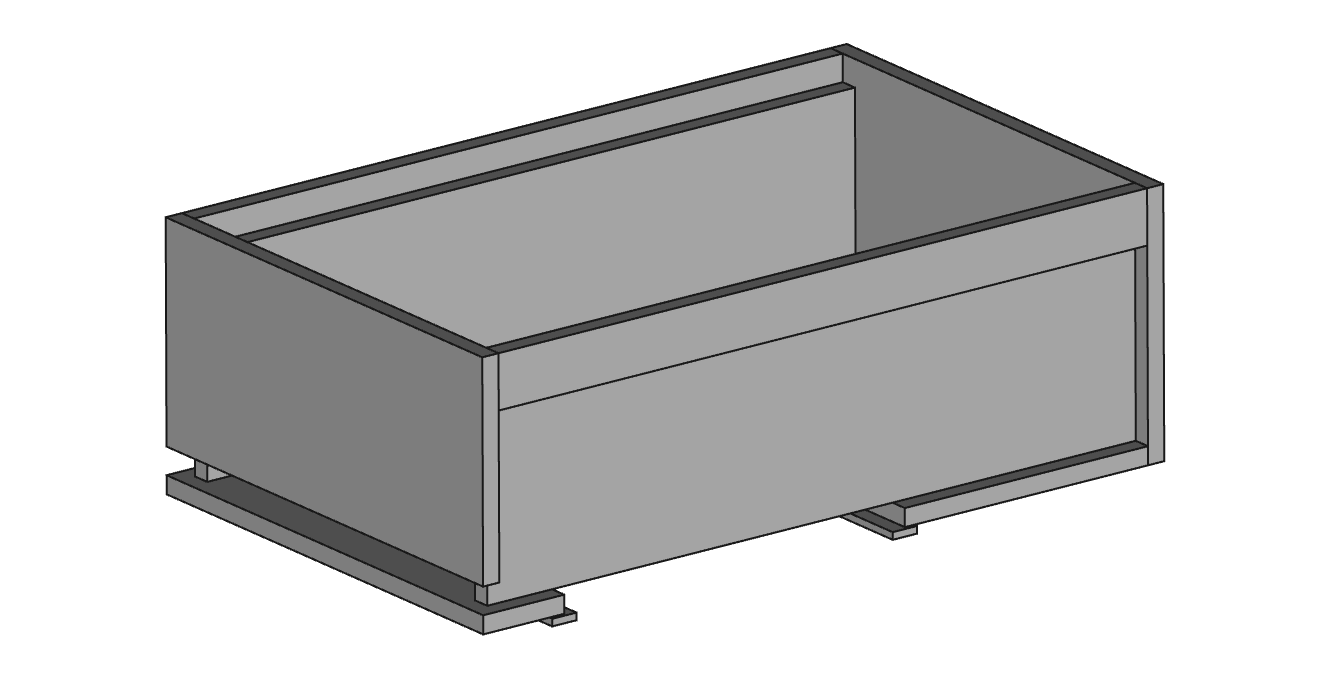
\includegraphics[width=\textwidth]{ansicht1}

[vgl. separate FreeCAD-Datei bzw. PDF-Pläne für konstruktive Details.]

\minisec{Teileliste}

\begin{center}
\begin{tabular}{lll}
  Bezeichnung &                       Maße [in mm] &          Anzahl \\
  \hline
  Seitenbrett links + rechts &        800 x 240 &             2 \\
  Seitl. Griffbrett links + rechts &  800 x 60 &              2 \\
  Stirnbrett vorne &                  540 x 240 &             1 \\
  Rückwand &                          540 x 290 &             1 \\
  Bodenbrett hinten &                 540 x 300 &             1 \\
  Bodenbrett vorne &                  540 x 100 &             1 \\
  Schubleisten &                      540 x 30 x 8 &          2 \\
  \hline
  Innendeckel (Dämmmaterial) &        850 x 540 &             1 \\
  \hline
\end{tabular}

[Materialstärke 25mm wenn nicht angegeben.]
\end{center}


\minisec{Zusatzteile}

\begin{itemize}
\item vertikales Königinnenabsperrgitter
\item vertikale Bienenflucht
\end{itemize}


\section{Offene Fragen}

\begin{enumerate}
%\item Boden: Öffnungen wegen Belüftung und besserer Varroabeobachtung? Oder reicht die Zugänglichkeit über das Flugloch?
%  (Stabilität der Konstruktion)
\item Notwendigkeit des Abspergitters: evtl. unnötig wg. des natürlichen Triebs der Königin, das Brutnest fluglochnah zusammenzuhalten?
\end{enumerate}


\section{Betriebsweise}

\subsection{Varroa: Winterbehandlung mit Oxalsäureverdampfer}

(Idee: Einblasloch im Fluglochstück? Entwicklung eines Verdampfers auf Basis eines Gasbrenners?)


\subsection{Ablegerbildung}

Entweder Bildung in der GSB (mit Fluglochverkleinerung und Volumenbegrenzungsschied)
oder in normalem Zander-Ablegerkasten


\subsection{Honigernte}

Benutzung des vertikalen Absperrgitters

vertikale Bienenflucht


\subsection{Varroa: Sommerbehandlung mit Ameisensäure}

Nassenheider Professional im bisherigen Honigraum


\subsection{Einfütterung}

Eimer im Honigraum


\section{Chronologie}

\begin{description}
\item[Herbst 2017] erste Vorüberlegungen
\item[Januar/Februar 2018] Planskizze
\item[Imkersaison 2018] Erprobungsbetrieb in Gersheim
\end{description}


\section{Literaturhinweise}

\begin{enumerate}
\item Gerhard Liebig, Einfach imkern, (3. Aufl.) 2011.
\item Friedrich Pohl (Hg.), Bienenkiste, Korb und Einfachbeuten. Naturnah und erfolgreich imkern, Stuttgart 2013.
\item Johannes Weber, Bienen halten mit der BienenBox, Stuttgart 2016.
\item Vinzenz Weber, Leichter imkern mit Trogbeuten, München (2. Aufl.) 1990.
\end{enumerate}
\end{document}